% LaTeX dokumentu guztiak zein dokumentu mota den adieraziz hasi behar dira
\documentclass[es]{ifirak}

% ERABILIKO DIREN PAKETEAK %

% listings paketea kodea formateatzeko erabiltzen da
\usepackage{listings}
% Paquete para los acentos
\usepackage[utf8]{inputenc}
\usepackage{pdfpages}
\usepackage{wrapfig}
\usepackage{amsmath}

 \usepackage{pdflscape}

% Paketea konfiguratu behar dugu C lengoaiarekin erabiltzeko:
\definecolor{darkgreen}{rgb}{0,0.5,0}
\definecolor{lightgray}{rgb}{0.95,0.95,0.95}
\definecolor{gray}{rgb}{0.65,0.65,0.65}
\lstset{language=C,
		basicstyle=\scriptsize\ttfamily,
		keywordstyle=\color{darkgreen}\bfseries,
		identifierstyle=\color{blue},
		commentstyle=\color{gray}, 
		stringstyle=\ttfamily,
		showstringspaces=false,
		tabsize=2,
		backgroundcolor=\color{lightgray}}


\begin{document}
% Hainbat datu ...
\ikasturtea{2014 - 2015}
\irakasgaia{Minería de Datos}
% Titulua
\title{Cuadernillo de prácticas}
% Zuen izena
\author{Mikel Dalmau}

% Abstract ingurunea hasierako laburpena idazteko erabili
\begin{abstract}
El siguiente documento está compuesto por una serie de prácticas realizadas en la asignatura de Minería de Datos, meta-clasificadores, selección de variables, predicción de nuevos casos, clusters, y sistemas de recomendación son los temas que se abordan, el software utilizado para las pruebas es Weka.
\end{abstract}

% Testua egituratzeko section, subsection, subsubsection, subsubsection eta paragraph komandoak dituzue
\section{Combinación de clasificadores }
\paragraph{}
La combinación de clasificadores es un campo de moda actualmente en el mundo del “machine learning”, el objetivo de esta practica es introducir las distintas clases de combinaciones, estudiar su funcionamiento y trabajar con ellas en Weka.
\subsection{Esquemas de combinación y sus parámetros}

\paragraph{}
\textbf{Boosting (Freund y Shapire, 1997):} Boosting es una meta algoritmo de clasificación para aprendizaje supervisado y sirve mayormente para reducir el error por sesgo, esto es, nunca se tiene una visión completa de que condiciona la clase y toda clasificación está sesgada en este sentido. Lo que hace es inducir clasificadores tomando cada vez una muestra más del conjunto de datos, inicialmente es equiprobable que una muestra sea seleccionada pero según avanza el algoritmo las muestras que fallan en la clasificación adquieren más peso y es más probable que sean reelegidas para una siguiente clasificación.
\paragraph{}
\textbf{Parámetros de AdaBoost(Boosting) en Weka}
\begin{itemize}
\item\textbf{Num Iterations:} Número de iteraciones que realizará el algoritmo.
\item\textbf{Classifier:} Clasificador a utilizar en el algoritmo, este algoritmo utiliza un sólo clasificador.
\item\textbf{Seed:} Cuando el clasificador base no puede tratar directamente con los pesos, la reselección se hace aleatoriamente utilizando la semilla indicada.
\item\textbf{Weight Threshold:} Este parámetro indica un mínimo de peso para que los casos sean seleccionados, estos es, los casos que el clasificador siempre clasifica correctamente cuando alcanzan ese mínimo de peso ya no se vuelven a seleccionar.
\item\textbf{Use Resampling:} Todo el proceso de asignación de peso se omite por una selección 
aleatoria.
\item\textbf{Debug:} El clasificador puede proporcionar información adicional por la consola.
\end{itemize}
\paragraph{}
\textbf{Bagging (Breiman, 1994):} Bagging o también Bootstrap aggregating es un meta algoritmo se utiliza para mejorar la estabilidad de algoritmos de clasificación, reduciendo la varianza e impidiendo la sobre adaptación a los datos. El algoritmo toma muestras de un conjunto de datos, que son combinaciones con reemplazo, e induce un modelo a partir de cada muestra. Finalmente se seleccionan los casos más votados.
\paragraph{}
\textbf{Parámetros de Bagging en Weka}
\begin{itemize}
\item\textbf{bagSizePercent:} Tamaño de cada selección en forma de porcentaje del conjutno de entrenamiento.
\item\textbf{calcOutOfBag:} Cada muestra de bootstrap deja fuera aproximadamente el 37\% de los ejemplos. Estos ejemplos pueden ser usados para formar estimaciones precisas de valores importantes. Por ejemplo, pueden ser utilizados para mejorar las estimaciones de probabilidades de nodos y nodo de error en los árboles de decisión. También pueden ser usados para dar estimaciones casi óptimas de los errores de generalización para predictores embolsados.
\end{itemize}
\paragraph{}
\textbf{Naive Bayes Tree:} Este clasificador híbrido compuesto induce árboles y en cada una de sus hojas tiene un clasificador Naive Bayes que se utilizará cuando alguno de los casos alcance 
dicha hoja. En Weka tiene como nombre NBTree y no requiere ningún parámetro más que la opción debug.
\paragraph{}
\textbf{Random Forest (Breiman, 2001):} Un random forest es un clasificador que consiste en una colección de clasificadores con estructura de árbol ${h(x, \Theta k ), k = 1,...}$ donde$ {\Theta k }$ son vectores aleatorios idénticamente distribuidos y cada árbol produce un único voto a la clase más popular para la entrada x.

\paragraph{}
\textbf{Parámetros de Random Forest en Weka}
\begin{itemize}
\item\textbf{Num Trees:} Número de árboles $h(x, \Theta k )$ a construir.
\item\textbf{Num Features:} Este es el parámetro que representa el valor k de la definición anterior, y representa el tamaño del vector aleatorio, en Weka representa el número de variables o atributos a escoger en cada dato y también podría representar el número de datos a escoger en cada árbol.
\end{itemize}
\paragraph{}
\textbf{Vote:}Una vez que varios clasificadores distintos han hecho una clasificación de un dato se selecciona como definitivo el valor de la clase que más votada.
\paragraph{}
\textbf{Parámetros de Vote en Weka}
\begin{itemize}
\item\textbf{Classifiers:} Una lista de clasificadores, al menos uno.
\item\textbf{Combination Rule:} Vote ofrece una serie de opciones para combinar los clasificadores, entre estas están, Majority Vote que sólo es válida para clases nominales minimum y maximum probability, average y product of probabilities, y finalmente median que sólo sirve con clases numéricas.
\end{itemize}
\paragraph{}
\textbf{Stacking:} Este es un meta clasificador en dos niveles,  un primer nivel formado por un conjunto de clasificadores distintos, para cada caso a clasificar, los resultados de estos clasificadores formarán las variables de un nuevo caso. En el segundo nivel otro clasificador utilizará estas evidencias para clasificar nuevamente.

\subsection{Resultados de aplicar los esquemas anteriores}

\begin{table}[htbp]
	\centering
	\begin{tabular}{l|c|r|}
		Clasificador & \% Acierto & Parámetros \\
		\hline
		J48 & 73.8281 & \\
		AdaBoost &  72.3958  & J48 numItr=10 WThreshold=100 \\
		Bagging & 74.6094 &\\
		Random Forest  & 75.3906 & Num Features=0 Num Trees=200 \\
		Random Forest  & 75.7813 & Num Features=2 Num Trees=200 \\
		Naive Bayes Tree  & 73.5677 &\\
		Vote  & 73.4375 & IB-2+J48+NB, majorityVote \\
		Stacking  & 74.8698 & IB-1+J48+NB $\rightarrow$ NB \\
		Stacking  & 74.7396 & IB-1+J48+NB+RF+RT $\rightarrow$ J48  \\
	\end{tabular}
	\caption{Resultados en la base de datos diabetes}\label{table}
\end{table}

\paragraph{}
Los resultados obtenidos en la base de datos diabetes han sido todos muy parecidos, la diferencia de utilizar meta-clasificadores no ha sido apreciable.

 En cualquier caso los resultados utilizando Random Forest han sido los mejores, esto es, los que utilizan combinaciones de un mismo clasificador base.

Puede ser que el número de casos de la base de datos 768 sea demasiado alto para que se note una mejora considerable al utilizar meta clasificadores.

 Si ha sido notable en cambio la diferencia en tiempos de computo entre unos algoritmos y otros, costando alrededor de un segundo por cada fold en los algoritmos con mayor cantidad de computo como el random forest, vote o Stacking. 

\begin{table}[htbp]
	\centering
	\begin{tabular}{l|c|r|}
		Clasificador & \% Acierto & Parámetros \\
		\hline
		J48 & 83.871 & \\
		AdaBoost &  85.8065  & J48 numItr=10 WThreshold=100 \\
		Bagging & 81.2903 &\\
		Random Forest  & 85.1613 & Num Features=0 Num Trees=200 \\
		Random Forest  & 86.4516 & Num Features=2 Num Trees=200 \\
		Naive Bayes Tree  & 82.5806 &\\
		Vote  & 82.5806 & IB-2+J48+NB, majorityVote \\
		Stacking  & 83.871 & IB-1+J48+NB $\rightarrow$ NB \\
		Stacking  & 79.3548 & IB-1+J48+NB+RF+RT $\rightarrow$ J48  \\
	\end{tabular}
	\caption{Resultados en la base de datos hepatitis}\label{table}
\end{table}

\paragraph{}
En la base de datos hepatitis también han sido homogéneos los resultados, el número de casos es bastante menor que en diabetes siendo este 155. Lo más notable de todo es la bajada en el porcentaje de acierto al utilizar el clasificador stacking.

Otra vez los mejores resultados los han dado los meta clasificadores que combinan un mismo clasificador base, AdaBoost y RandomForest.

\begin{table}[htbp]
	\centering
	\begin{tabular}{l|c|r|}
		Clasificador & \% Acierto & Parámetros \\
		\hline
		J48 & 63.4921 & \\
		AdaBoost &  63.4921  & J48 numItr=10 WThreshold=100 \\
		Bagging & 52.381 &\\
		Random Forest  & 69.8413 & Num Features=0 Num Trees=200 \\
		Random Forest  & 68.2540 & Num Features=2 Num Trees=200 \\
		Naive Bayes Tree  & 57.1429 &\\
		Vote  & 63.4921 & IB-2+J48+NB, majorityVote \\
		Stacking  & 50.7937 & IB-1+J48+NB $\rightarrow$ NB \\
		Stacking  & 53.9683 & IB-1+J48+NB+RF+RT $\rightarrow$ J48  \\
	\end{tabular}
	\caption{Resultados en la base de datos white clover}\label{table}
\end{table}

\paragraph{}
Esta última base de datos tiene todavía menos casos que las anteriores, cuenta con 63, pero cada caso en cambio tiene 31 atributos distintos siendo la mayoría reales excepto 3 nominales.

Esta vez las diferencias en porcentaje de acierto entre unos clasificadores y otros son bastante notables llegando casi al 20\%.

Otra vez, al igual que en el caso anterior los peores resultados se obtienen al utilizar Stacking, he probado a añadir muchos clasificadores base y cambiar  el de mayor nivel y los resultados no mejoran, sospecho que el motivo es que al tratarse de un clasificador en dos niveles el ajuste a los datos de entrenamiento es menor, y por eso los porcentajes de acierto baja, aunque si esto es así también significaría que posiblemente Stacking sigiera obteniendo resultados aceptables con casos diferentes de los del conjunto de entrenamiento mientras el resto de algoritmos fallan, aunque no estoy del todo seguro de esto último.

\section{Problemas “benchmark” de clasificación}
\paragraph{}
Hoy en día, cuando se publica un estudio en el mundo de la investigación de la minería de datos no pueden presentarse resultados en cualquier base de datos, es necesario utilizar alguna de las bases de datos públicas reconocidas por la comunidad, un repositorio famoso es el UCI machine learning repository de la universidad de California Irvine. Esta práctica consiste en exponer una de estas bases de datos públicas y responder a una serie de preguntas en relación a otra base de datos obtenida en el portal kdnuggets.com.

\subsection{Demospongiae data set}
\paragraph{}
El siguiente problema de clasificación supervisada consiste reconocer la familia u orden de una esponja marina. El conjunto de datos contiene 503 esponjas de la clase Demospongiae recogidas la mayoría en el Mediterráneo (451) y algunas en el Atlántico (52). Cada esponja se clasifica de acuerdo a la siguiente jerarquía: orden, familia, género y especie. De esta forma cada orden está subdividido en varias familias, las cuales están divididas en varios géneros y cada género en varias especies. 

\begin{wrapfigure}{r}{0.4\textwidth}
	\begin{center}
		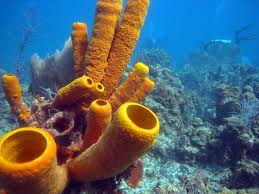
\includegraphics[width=0.35\textwidth]{telechargement.png}
	\end{center}
	\caption{Esponja marina}
	\vspace{-50pt}
\end{wrapfigure}

\paragraph{}
Aunque se puede clasificar en cualquiera de estos niveles, típicamente se utiliza la clase orden ya que la base de datos no tiene el tamaño suficiente para clasificar las otras con precisión y exactitud.
\paragraph{}
En la base de datos la distribución y número de clases es la siguiente
\begin{itemize}
\item 7 ordenes differentes (de 42 a 117 esponjas por orden)
\item 42 familias diferentes (de 1 a 43 esponjas por familia)
\item 114 géneros diferentes (de 1 a 34 esponjas por género)
\item 230 especies diferentes (de 1 a 15 esponjas por especie)
\end{itemize}

\paragraph{}
Las variables clase anteriormente expuestas toman valores nominales, el nombre científico de dicho orden o  familia, por ejemplo, astrophoricda, axinellida y hadromerida son entre otros tres valores que puede tomar la clase orden. 
Vistos en mínimo y máximo de casos por clase podemos decir que el problema está bastante balanceado, al menos para orden.

\begin{figure}[htbp]
	\centering
	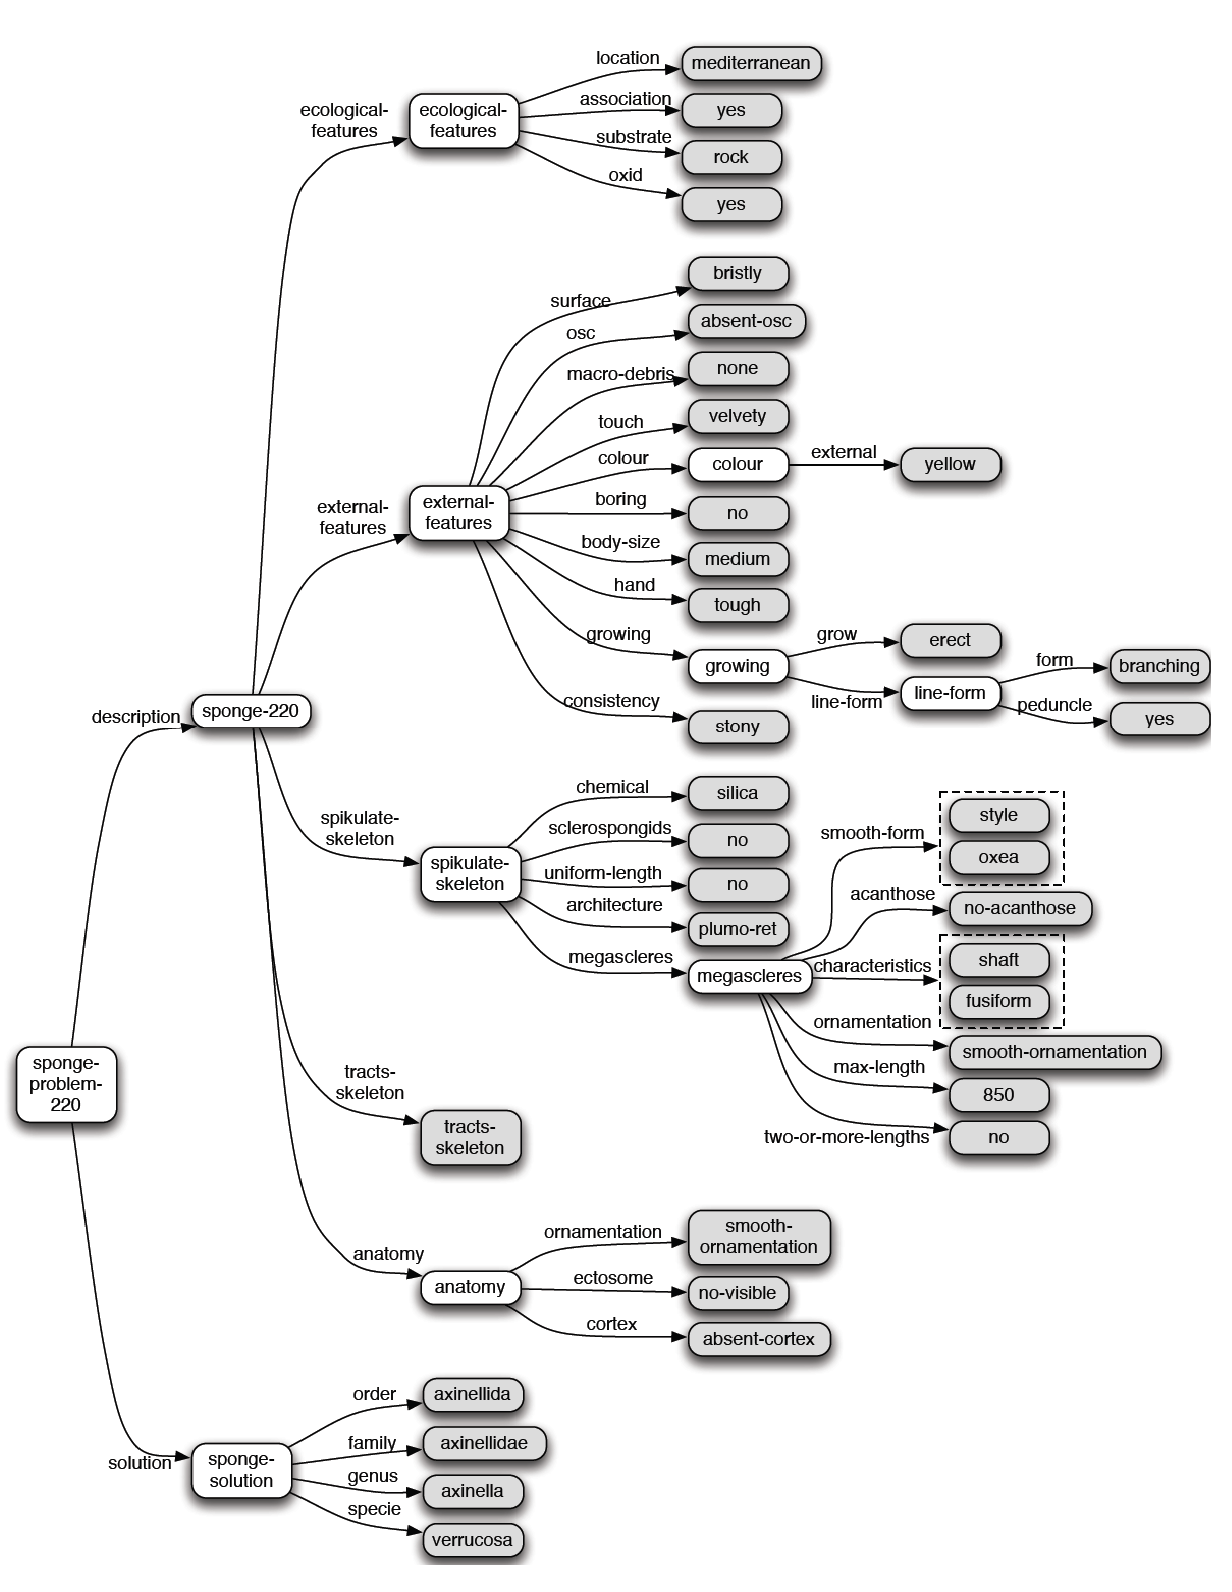
\includegraphics[width=1\textwidth]{Esquema.png}
	\caption{Esquema de clasificación, variables predictoras y clases}\label{figure}
\end{figure}

\paragraph{}
La base de datos cuenta con 30 variables predictoras, estas están divididas en grupos según de que tipo sean, si hacen referencia a la esponja en sí o a su habitat, a su esqueleto, su anatomía y sus atributos tales como el color o el tacto.

\paragraph{}
El siguiente esquema muestra las variables predictoras y las clases para una esponja concreta.

\paragraph{}
Me ha llamado la atención esta base de datos entre las otras en primer lugar por el tema, siempre me ha interesado la naturaleza, podríamos pensar que una base de datos como esta no tiene ningún interes ni aplicación en la vida real, pero creo que si alguna vez se inventara un robot que tuviera que reconocer animales, marinos en este caso o bien podrían ser terrestres, sería muy util para él disponer de un esquema de clasificación y un conjunto de entrenamiento como este.

\subsection{Google n-grams}
\paragraph{}
He escogido esta base de datos en primer lugar porque ha sido creada por google, y he pensado que si google la ha hecho debería ser importante, también me ha llamado la atención la descripción expuesta en kdnuggets en la que dice "texto de un millon de libros escaneados por google", aunque no es una descripción muy representativa de los datos almacenados.
\paragraph{}
Esta base de datos es ingente y está subdividida en numerosos ficheros dependiendo principalmente del idioma, estan incluidos el inglés, francés, chino, aleman, ruso, hebreo, italiano y español. El siguiente nivel de división está definido por el tamaño de los n-gramas. Un n-grama es una subsecuencia de n elementos de una secuencia dada, podemos encontrar desde 1-gramas hasta 5-gramas en las bases de datos de google. Existe todavía otra subdivisión de archivos, en el siguiente nivel se separan los n-gramas según el caracter o número de comienzo.

\paragraph{}
Por ejemplo, estas son las líneas 3.000.000 y 3.000.001 de un archivo de los 1-gramas para el inglés. La primera línea nos dice que la palabra circumvallate aparece 335 veces en 91 libros diferentes durante el año 1978.\\
circumvallate   \hspace{0.7cm}1978   \hspace{0.7cm}335 \hspace{0.7cm}   91\\
circumvallate   \hspace{0.7cm}1979 \hspace{0.7cm}261  \hspace{0.7cm}  91 

\paragraph{}
Esta sería la línea 9,000,000 del archivo 0 de los 5-gramas para el inglés, esta vez aparece un nuevo atributo que indica la página en la que aparece la secuencia.\\
analysis is often described as \hspace{0.7cm} 1991 \hspace{0.7cm} 1 \hspace{0.7cm} 1 \hspace{0.7cm} 1

\paragraph{}
El estudio de los n-gramas es interesante en diversas áreas del conocimiento. Por ejemplo, es usado en el estudio del lenguaje natural, en el estudio de las secuencias de genes y en el estudio de las secuencias de aminoácidos. Se puede usar gramas para casi todos los ámbitos. Por ejemplo, se han usado n-gramas para extraer características comunes de grandes conjuntos de imágenes de la Tierra tomadas desde satélite, y para determinar a qué parte de la Tierra pertenece una imagen dada.\\

En nuestro caso, teniendo en cuenta que google ha utilizado libros para extraer los n-gramas, los más apropiado sería utilizarlos para el procesamiento del lenguaje natural.\\

Por ejemplo podríamos utilizar los 4-gramas o 5-gramas para conocer las frecuencia de aparición de ciertas frases hechas a lo largo de los años y así tratar de predecir si caerán en desuso o al contrario se harán populares.\\

También podríamos utilizarlos para encontrar candidatos probables para la correcta ortografía de una palabra mal escrita.Por ejemplo:\\

...el cazador disparar(disparó) al animal...\\

Un procedimiento posible, grosso modo, podría ser el siguiente, buscamos el 2-grama (cazador disparar) y como es incorrecto habrá muy pocos 2-gramas o ninguno como ese por lo que nuestro programa sabrá que alguna de las dos palabras no es correcta en cambio (el cazador) si que es correcto y parece un 2-grama bastante común por lo que el programa sabrá que el fallo está es disparar y no en cazador, luego podemos buscar 2-gramas con la palabra cazador y la raiz disp- en la seguna palabra y seleccionar la más común. \\


Finalmente los n-gramas están separados por saltos de línea y los atributos de cada línea por tabulaciones por lo que extraer los datos para crear otro tipo de archivo no debería ser demasiado complicado y podría utilizarse casi cualquier lenguaje de programación, ahora, el número de casos por fichero es ingente y muy variable ya que no existe el mismo número de palabras que comienzan con a que con x por ejemplo, entre los archivos que he podido abrir (los más pequeños) había alrededor de 15 millones de casos.

\section{Predicción de la clase de casos nuevos sin etiquetar -- "Class prediction"}
\paragraph{}
El objetivo de esta práctica es predecir la clase de casos futuros de los cuales desconocemos su etiqueta-clase verdadera.\\

Para realizarla he elegido la base de datos diabetes.arff, el objetivo de la base de datos es predecir si un paciente tiene diabetes o no según las siguientes variables.
\begin{enumerate}
	\item Number of times pregnant
	\item Plasma glucose concentration a 2 hours in an oral glucose tolerance test
	\item Diastolic blood pressure (mm Hg)
	\item Triceps skin fold thickness (mm)
	\item 2-Hour serum insulin (mu U/ml)
	\item Body mass index $(weight in kg/(height in m)^2)$
	\item Diabetes pedigree function
	\item Age (years)
	\item Class variable (0 or 1)
\end{enumerate}
\paragraph{}
Luego he añadido al final de la base de datos los siguientes casos sin etiqueta clase, notese el signo de interrogación en el campo correspondiente a la clase.
	
\begin{itemize}
	\item 0,50,60,5,0,25.3,0.109,20,?
	\item	1,70,65,10,15,31.4,0.221,30,?
	\item	2,90,70,15,30,36.9,0.900,50,?
	\item	3,130,75,20,400,41.1,0.001,90,?
	\item	8,200,95,30,300,46.3,0.075,110,?
\end{itemize}

\textbf{Output predictions para los clasificadores Naive Bayes y 10-NN}

\begin{table}[htbp]
		\centering
		\begin{tabular}{|c|c|l|c|c|}
			inst &   actual    & predicted   & error & probability  distribution \\ \hline
			764  & 1:tested\_n & 2:tested\_p &   +   &    0.312    \hspace{0.4cm}    *0.688    \\
			765  & 1:tested\_n & 1:tested\_n &       &   *0.896    \hspace{0.4cm}    0.104     \\
			766  & 1:tested\_n & 1:tested\_n &       &   *0.928   \hspace{0.4cm}     0.072     \\
			767  & 2:tested\_p & 1:tested\_n &   +   &   *0.858   \hspace{0.4cm}     0.142     \\
			768  & 1:tested\_n & 1:tested\_n &       &   *0.995   \hspace{0.4cm}     0.005     \\
			769  &      ?      & 1:tested\_n &   +   &   *0.994   \hspace{0.4cm}     0.006     \\
			770  &      ?      & 1:tested\_n &   +   &   *0.98   \hspace{0.4cm}      0.02     \\
			771  &      ?      & 1:tested\_n &   +   &   *0.798   \hspace{0.4cm}     0.202     \\
			772  &      ?      & 2:tested\_p &   +   &    0.039   \hspace{0.4cm}    *0.961    \\
			773  &      ?      & 2:tested\_p &   +   &    0.001    \hspace{0.4cm}   *0.999
		\end{tabular}
	\caption{Resultados para Naive Bayes }\label{table}
\end{table}

\begin{table}[htbp]
	\centering
	\begin{tabular}{|c|c|l|c|c|}
		inst &   actual    & predicted   & error & probability  distribution \\ \hline
		764  & 1:tested\_n & 1:tested\_n &       &       *0.7  \hspace{0.4cm}   0.3        \\
		765  & 1:tested\_n & 1:tested\_n &       &        *0.9   \hspace{0.4cm} 0.1        \\
		766  & 1:tested\_n & 1:tested\_n &       &       *0.8   \hspace{0.4cm}   0.2       \\
		767  & 2:tested\_p & 2:tested\_p &       &        0.4   \hspace{0.4cm} *0.6        \\
		768  & 1:tested\_n & 1:tested\_n &       &        *1    \hspace{0.4cm}   0         \\
		769  &      ?      & 1:tested\_n &   +   &         *1   \hspace{0.4cm}   0         \\
		770  &      ?      & 1:tested\_n &   +   &        *1    \hspace{0.4cm}    0        \\
		771  &      ?      & 1:tested\_n &   +   &        *0.7  \hspace{0.4cm}  0.3        \\
		772  &      ?      & 1:tested\_n &   +   &        *0.6  \hspace{0.4cm}  0.4        \\
		773  &      ?      & 2:tested\_p &   +   &        0.2  \hspace{0.4cm}*0.8
	\end{tabular}
	\caption{Resultados para 10-NN }\label{table}
\end{table}

\paragraph{}
Las anteriores dos tablas muestran los resultados predichos por ambos clasificadores para los últimos 10 casos de la base de datos, icluidos los últimos 5 añadidos que no tienen clase.\\

Las columnas de la tabla significan lo siguiente:

\begin{itemize}
	\item \textbf{inst:} Este valor indica el número del caso en cuestión, como hemos añadido los casos nuevos al final podemos ver que la base de datos tenía 768 casos originalmente.
	\item	\textbf{actual:} Valor real de la clase, podemos ver que es interrogante en los casos si etiquetar tal y como era de esperar.
	\item	\textbf{predicted:} Valor de la clase predicho por el clasificador.
	\item	\textbf{error:} Es positivo cuando la clase predicha no coincide con la real, en los casos sin etiquetar siempre será positivo ya que no conocemos el valor real de la etiqueta.
	\item	\textbf{probability distribution:} La última columna incluye dos valores en cada fila, el primero de los valores representa la probabilidad según el modelo aprendido de que el caso se clasificado como negativo, el segundo la probabilidad de que sea clasificado como positivo, el asterisco indica el de mayor probabilidad y el elegido por el modelo. Si nuestra clase tuviera mas de dos valores posibles las columnas serían tantas como valores diferentes pudiera adoptar la clase pero la suma de cada fila será siempre 1.
	\paragraph{}
	Hablo de probabilidad a priori en el caso de naive bayes ya que se trata de un algoritmo entusiasta y no podemos utilizar esos casos para aprender el modelo (por falta de clase), una vez aprendido el modelo lo utilizamos para clasificar los nuevos casos, en el caso de los vecinos más cercanos la probabilidad se calcula localmente en el momento de aprender el clasificador por lo que no se trata de una probabilidad a priori.
	\paragraph{}
	La primera diferencia entre los valores de probabilidad obtenidos en las dos tablas es que los valores para 10-NN no tiene más de un decimal, esto tiene todo el sentido del mundo si tenemos en cuenta el valor k seleccionado, si en vez de 10-NN hubieramos elegido 2-NN los valores de probabilidad posibles serían 0,1 y 0.5 esto es, dependerá del número y los valores de la clase de los vecinos más cercanos.
\end{itemize}
\pagebreak
\section{Selección de variables}
\paragraph{}
Como bien sabemos, en un problema de clasificación la relevancia de todas las variables predictoras de la base de datos no es la misma. Predictoras redundantes (entre ellas) y/o irrelevantes (sin relación respecto a la clase a predecir) pueden degradar la capacidad predictiva de los clasificadores. WEKA permite, mediante su funcionalidad-pestaña "Select Attributes", realizar numerosas tareas de selección de variables, con el fin de afrontar la futura construcción de los clasificadores con menos variables, y también con el objetivo de saber cuáles son las variables predictoras interesantes en el problema, y quizás también mejorar la capacidad predictiva\\

\textbf{Filter vs Wrapper}
\paragraph{}
El método wrapper se caracteriza por valorar distintos subconjuntos de atributos utilizando el porcentaje de bien clasificados para un cierto modelo. Tiene la ventaja de encontrar normalmente el mejor subconjunto de atributos para el modelo utilizado aunque es computacionalmente costoso ya que tiene que entrenar un modelo distinto y validarlo para cada subconjunto, por otro lado el subconjunto encontrado podría no ser el mejor para otro algoritmo de clasificación.\\

El método filter, a diferencia de wrapper, establece una medida indirecta de la aportación de cada variable a la clasificación. De esta forma crea un ranking de variables según su correlación con la clase, luego se seleccionan las k variables más significativas. Aunque computacionalmente es menos costos que wrapper, no podemos saber que rendimiento tendrá el subconjunto elegido en el clasificador a usar, por eso, una práctica bastante extendida en problemas grandes es utilizar filter como etapa de pre-procesamiento seguido del método wrapper.\\

\textbf{white clover .arff}\\

Para trabajar en esta práctica hemos seleccionado la base de datos white clover, que trata un problema de clasificación supervisada donde se pretende determinar la población de una especie de hierba en un lugar concreto dependiendo de la población de esa misma especie y otras especies durante los años anteriores, cada caso cuenta con 31 variables predictoras.\\

\textbf{Chi Cuadrado }
\paragraph{}
Para realizar filter he utilizado 10-fold cross validation, la columna izquierda es la media de valores obtenidos junto con la desviación típica, weka muestra además una columna extra que he omitido con la media de los puestos obtenidos en el ranking.\\

La Distribución chi-cuadrado tiene por función de densidad la siguiente, donde el parámetro $k$ de  $\chi^2_k$ , se denomina grados de libertad de la distribución y $\varGamma$ es la función gamma.

\begin{displaymath}
	\chi^2_k,=, \dfrac{x^{k/2-1}e^{-x/2}}{2^{k/2}\varGamma(k)}
\end{displaymath}

La tabla 6 muestra el ranking obtenido en weka tras utilizar el método filter con el estadístico chi-cuadrado, hay una serie de valores que han obtenido puntuación 0, esto puede ser que esos valores no tienen ningún efecto directo sobre la variable clase no reducen la entropía de la clase una, lo sorprendente es encontrar valores distintos de 0 con ranking peores que 0.\\
\pagebreak
\begin{table}[htbp]
	\centering
	\begin{tabular}{|c|rl|}
		  Puntuación    & Variable Predictora &  \\ \hline
		33.395 +- 7.245 &  27 OtherGrasses-94 &  \\
		29.116 +- 3.811 &            1 strata &  \\
		13.134 +- 1.513 &           3 paddock &  \\
		30.7   +-20.522 &      29 RyeGrass-94 &  \\
		7.048 +- 1.294  &              2 plot &  \\
		4.788 +- 0.873  &  31 strata-combined &  \\
		  0     +- 0    &   8 OtherLegumes-91 &  \\
		  0     +- 0    &       9 RyeGrass-91 &  \\
		  0     +- 0    &         10 Weeds-91 &  \\
		  0     +- 0    &   7 OtherGrasses-91 &  \\
		  0     +- 0    &    12 BareGround-92 &  \\
		3.073 +- 6.146  &   11 WhiteClover-92 &  \\
		  0     +- 0    &      6 Cocksfoot-91 &  \\
		  0     +- 0    &     5 BareGround-91 &  \\
		  0     +- 0    &    25 BareGround-94 &  \\
		  0     +- 0    &  28 OtherLegumes-94 &  \\
		  0     +- 0    &     26 Cocksfoot-94 &  \\
		  0     +- 0    &    4 WhiteClover-91 &  \\
		  0     +- 0    &         24 Weeds-93 &  \\
		  0     +- 0    &     13 Cocksfoot-92 &  \\
		  0     +- 0    &      23 RyeGrass-93 &  \\
		4.686 +- 7.194  &         30 Weeds-94 &  \\
		  0     +- 0    &  22 OtherLegumes-93 &  \\
		  0     +- 0    &  21 OtherGrasses-93 &  \\
		  0     +- 0    &  14 OtherGrasses-92 &  \\
		  0     +- 0    &     20 Cocksfoot-93 &  \\
		  0     +- 0    &    19 BareGround-93 &  \\
		  0     +- 0    &  15 OtherLegumes-92 &  \\
		  0     +- 0    &   18 WhiteClover-93 &  \\
		2.193 +- 6.579  &      16 RyeGrass-92 &  \\
		  0     +- 0    &         17 Weeds-92 &
	\end{tabular}
	\caption{Filtro utilizando estadístico chi-cuadrado sobre la base de datos white clover}\label{table}
\end{table}
\pagebreak

\textbf{Gain ratio}
\paragraph{}
La tabla 7 muestra el ranking obtenido en weka tras utilizar el método filter con el evaluador gain ratio, que valora los atributos según el ratio de ganancia que tienen con respecto a la clase

\begin{displaymath}
GainR(Class, Attribute) =\dfrac {H(Class) - H(Class | Attribute)}{H(Attribute)}
\end{displaymath}

\begin{table}[htbp]
	\centering
	\begin{tabular}{|c|rl|}
		  Puntuación   & Variable Predictora &  \\ \hline
		0.35  +- 0.03  &  27 OtherGrasses-94 &  \\
		0.123 +- 0.014 &            1 strata &  \\
		0.116 +- 0.014 &           3 paddock &  \\
		0.585 +- 0.387 &      29 RyeGrass-94 &  \\
		0.058 +- 0.012 &              2 plot &  \\
		0.059 +- 0.009 &  31 strata-combined &  \\
		  0     +- 0   &       9 RyeGrass-91 &  \\
		  0     +- 0   &         10 Weeds-91 &  \\
		  0     +- 0   &   7 OtherGrasses-91 &  \\
		  0     +- 0   &   8 OtherLegumes-91 &  \\
		0.024 +- 0.071 &   11 WhiteClover-92 &  \\
		  0     +- 0   &      6 Cocksfoot-91 &  \\
		  0     +- 0   &     26 Cocksfoot-94 &  \\
		  0     +- 0   &    25 BareGround-94 &  \\
		  0     +- 0   &  28 OtherLegumes-94 &  \\
		  0     +- 0   &     5 BareGround-91 &  \\
		  0     +- 0   &    12 BareGround-92 &  \\
		  0     +- 0   &    4 WhiteClover-91 &  \\
		0.046 +- 0.137 &      23 RyeGrass-93 &  \\
		  0     +- 0   &     13 Cocksfoot-92 &  \\
		  0     +- 0   &         24 Weeds-93 &  \\
		0.083 +- 0.127 &         30 Weeds-94 &  \\
		  0     +- 0   &  14 OtherGrasses-92 &  \\
		  0     +- 0   &  22 OtherLegumes-93 &  \\
		  0     +- 0   &  21 OtherGrasses-93 &  \\
		  0     +- 0   &  15 OtherLegumes-92 &  \\
		  0     +- 0   &     20 Cocksfoot-93 &  \\
		  0     +- 0   &    19 BareGround-93 &  \\
		  0     +- 0   &   18 WhiteClover-93 &  \\
		  0     +- 0   &         17 Weeds-92 &  \\
		  0     +- 0   &      16 RyeGrass-92 &
	\end{tabular}
	\caption{Filtro utilizando estadístico gain ratio sobre la base de datos white clover}\label{table}
\end{table}

\paragraph{}
En el siguiente dibujo podemos ver que los primeros y más importantes nodos del árbol generado por el algoritmo J48 de Weka no coinciden mucho con el ranking obtenido, sólo la variable RyeGrass-94 se encuentra entre las top del ranking y aunque tiene una puntuación muy alta la desviación típica es muy alta también, lo que indica que dependiendo del conjunto de entrenamiento varia mucho la puntuación obtenida.

\pagebreak

\begin{figure}[htbp]
	\centering
	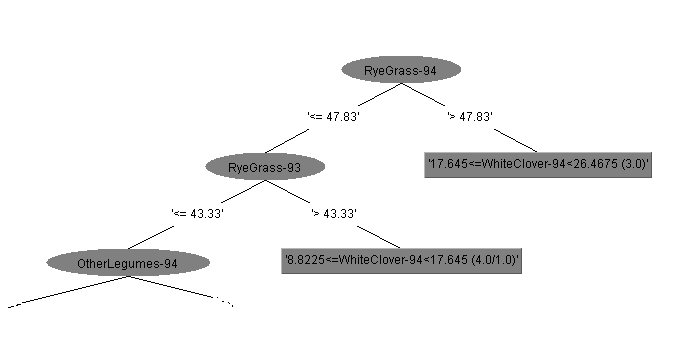
\includegraphics[width=0.6\textwidth]{J48Tree.png}
	\caption{Primeros tres nodos del árbol de decisión J48}\label{figure}
\end{figure}

Estas líneas son las reglas inducidas por el clasificador Jrip, vemos que las variables que utiliza el clasificador, en orden de relevancia, son RyeGrass-94, Weeds-94, plot y RyeGrass-93, siguiendo en la línea del árbol J48 que tiene RyeGrass-94 como raíz.
$$(RyeGrass-94 >= 50) => WhiteClover-94=17.645<=WhiteClover-94<26.4675 (3.0/0.0)$$
$$(Weeds-94 >= 17.82) => WhiteClover-94=8.8225<=WhiteClover-94<17.645 (21.0/8.0)$$
$$(plot = huia) and (RyeGrass-93 >= 17.95) => WhiteClover-94=8.8225<=WhiteClover-94<17.645 (6.0/0.0)$$
$$=> WhiteClover-94=0<=WhiteClover-94<8.8225 (33.0/3.0)$$
\paragraph{}
\textbf{Resultados k-NN tras reducción de variables predictoras}\\

Los siguientes resultados muestran una mejora del 6\% al utilizar el algoritmo 3-NN con las 5 variables más significativas pero una perdida del 4\% al utilizar las top 10, .\\

Porcentaje de acierto del clasificador 3-NN con todas las variables: 65.0794 \%\\

Porcentaje de acierto del clasificador 3-NN con las top 5 del ranking anterior (27 OtherGrasses-94, 1 strata, 3 paddock, 29 RyeGrass-94, 2 plot): 71.4286 \%\\

Porcentaje de acierto del clasificador 3-NN con las top 10 del ranking anterior: 61.9048\%\\

\paragraph{}
\textbf{Más comentarios}\\

Respecto a los rankins obtenidos anteriormente puede apreciarse que en ambos, aunque computen valores distintos, el orden de las variables es el mismo, esto es lógico ya que independientemente del método que utilicemos para hallar la relación entre la clase y una variable esa relación seguirá estando ahí y no va a cambiar.\\

Esta manera de seleccionar las mejores variables no garantiza la eliminación de variables redundantes ya que se analizan independientemente si no me equivoco. Para lograr esto, en el caso de gain ratio por ejemplo, podríamos tratar de hallar los pares de variables que no reducen la entropía mucho más que por sí solos, lo que indicaría que son variables redundantes.\\


\textbf{¿Cómo es posible que WEKA nos devuelva el nivel de correlación entre predictoras numéricas y la variable clase nominal? ¿Qué está haciendo WEKA? Puedes consultar en los foros, buscar en la Red...}
He buscado en la red sobre esto y no he encontrado nada, aunque en este caso la clase no es del todo nominal sino numérica y discretizada en cuatro intervalos por lo que es posible que Weka asigne el centro de cada intervalo como valor representativo. No se que podría suceder si la clase fueran colores o algun tipo nominal así.

\section{Clasificación no supervisada, “clustering” mediante “k-means”}

\paragraph{}
El problema que he escogido para esta practica trata de idiomas europeos, recoge los porcentajes de personas en cada país que dice ser capaz de hablar un idioma europeo. El interés de la base de datos puede ser hallar relaciones lingüísticas entre países, es lógico que países vecinos o con mucho contacto compartan un gran número de parlantes de sus idiomas respectivos, más allá de esto no se que tipo de interés podría tener.\\

La fecha de la base de datos es bastante antigua por lo que en muchos casos la información está desfasada, claro que hay otros datos que se mantendrán igual, por ejemplo el 100\% de la gente de España hablará español todavía pero seguramente el porcentaje de personas que hablan ingles habrá aumentado del 5\%.\\

Para transformar el fichero de texto a formato .arff lo he hecho manualmente tomando otro archivo .arff como modelo, los identificadores de las columnas(idioma) los he transformado en atributos numéricos, los identificadores de las filas(países) los he transformado en un único atributo nominal que sirve de identificador de cada fila, las filas de la matriz del archivo original se han transformado en una línea de weka cada una, luego he añadido las comas, quitado los espacios y cambiado los caracteres de comentario. Por suerte la base de datos es bastante sencilla y no me ha llevado demasiado tiempo esta transformación.\\

 
\textbf{Parámetros de SimpleKMeans en Weka}
\begin{itemize}
	\item \textbf{maxIterations:} Número de iteraciones máximo a realizar por el algoritmo.
	
	\item \textbf{distanceFunction:} Medida de distancia a utilizar para compara los casos, por defecto la Euclídea.
	
	\item \textbf{numClusters:} Número de clusters a crear.
	\item \textbf{displayStdDevs:} Mostrar las desviaciones estándar de atributos numéricos y el recuento de atributos nominales.
\end{itemize}

\textbf{Explica los siguientes conceptos}
\begin{itemize}
	\item  \textbf{number of iterations:} Tras varias ejecuciones el número de iteraciones ha sido 2 siempre, aunque el máximo es 500, esto significa que al algoritmo le basta con dos para cumplir el criterio de parada.
	
	\item \textbf{cluster centroids:} Distancia de los atributos a cada uno de los centroides, es esencial esta distancia para realizar el algoritmo kmeans. 
	\item \textbf{clustered instances:}  Aquí están indicadas cuantas instancias han sido asignadas a cada cluster.
	
\end{itemize}

\subsection{Análisis de clústering, Idiomas}

\begin{table}[htbp]
	\centering
	\begin{tabular}{|l|c|c|c|c|c|}
		Attribute &   Full Data   &   0    &       1       &   2    &       3        \\
		          &     (16)      &  (3)   &      (4)      &  (6)   &      (3)       \\ \hline
		country   & West\_Germany & Sweden & West\_Germany & Italy  & Great\_Britain \\
		FI        &    0.0629     & 0.0148 &    0.2406     &   0    &       0        \\
		SW        &    0.0961     & 0.4322 &    0.0553     & 0.0033 &       0        \\
		DA        &    0.0713     & 0.3705 &       0       & 0.0049 &       0        \\
		NO        &    0.0726     & 0.3872 &       0       &   0    &       0        \\
		EN        &    0.3256     & 0.3363 &    0.1902     & 0.1324 &     0.8819     \\
		GE        &    0.3076     & 0.2328 &    0.5912     & 0.2965 &     0.0263     \\
		DU        &    0.0456     & 0.0028 &    0.1682     & 0.0079 &       0        \\
		FL        &    0.0924     & 0.0028 &    0.1658     & 0.1345 &       0        \\
		FR        &    0.2721     & 0.0581 &    0.0647     & 0.5033 &     0.3004     \\
		IT        &    0.1029     & 0.0145 &    0.0154     & 0.2397 &     0.0343     \\
		SP        &     0.083     & 0.0058 &    0.0081     & 0.1853 &     0.0555
	\end{tabular}
	\caption{Resultados de k-means en Weka para 4 clusters}\label{table}
\end{table}

\begin{table}[htbp]
	\centering
	\begin{tabular}{c|c}
Clustered & Instances\\
\hline
0     &  3 ( 19\%)\\
1     &  4 ( 25\%)\\
2     &  6 ( 38\%)\\
3     &  3 ( 19\%)\\
	\end{tabular}
	\caption{Clustered instances}\label{table}
\end{table}
\paragraph{}
Esta configuración es la que más me convence porque he probado con otras y me gusta como ha quedado la distribución de casos en los clusters, es bastante homogénea y ningún cluster se ha quedado con un solo caso.\\

Entre las variables estudiadas las que hacen referencia a idiomas ampliamente hablados, como el inglés el alemán o el francés toman valores similares en todos los centroides, en cambio las que hacen referencia a idiomas poco hablados como los Nórdicos o el italiano toman valores lejanos respecto del resto de centroides.\\
\pagebreak

Algunos de los casos parece que no está en el cluster apropiado o estaría mejor en otro, por ejemplo esperaríamos que Portugal perteneciera a los Países Latinos o Finlandia a los Nórdicos. De todas formas el problema trata de idiomas y no es raro que hubiera más gente en Portugal que supiera inglés en vez de castellano o francés.\\

\textbf{Países en cada cluster}
\begin{enumerate}
	\item Sweden, Norway, Denmark \textbf{etiqueta:} Países Nórdicos.
	\item Italia, Francia, Belgica, Luxemburgo, Suiza, España \textbf{etiqueta:} Países Latinos
	\item Austria, West Germany, Netherlands, Finland \textbf{etiqueta:} Países Germanos
	\item Ireland, Great Britain, Portugal \textbf{etiqueta:} Gran Bretaña y alrededores
	
\end{enumerate}

\pagebreak

\subsection{Análisis de clustering, Esponjas}
\paragraph{}
Esta base de datos también trata de esponjas, en la línea con la expuesta en la anterior práctica, aunque ahora el número de casos es menor y todos los casos corresponden al mismo orden O.Hadromerida como todas las esponjas son del Mediterráneo es posible que esta base de datos haya sido extraída de la anterior.\\

El análisis de estos resultados es mucho más complicado que el anterior ya que no soy un experto en biología marina. Identificar las diferencias entre los clusters es mucho más difícil. De todas formas viendo los pequeños gráficos en dos dimensiones que ofrece el visualizador de clusters de Weka pueden distinguirse mejor las variables que toman valores más lejanos respecto de los centroides. Por ejemplo, la primera variable, las esponjas que no tienen capas de cortex están todas en el primer cluster y las que tienen 1, 2 o 3 capas están en el segundo cluster, no hay esponjas de color Azul o Naranja en el cluster 1.\\

Como ya he indicado antes, difícilmente voy a poder identificar los clusters con familias de esponjas diferentes y comprobar que efectivamente el algoritmo opera satisfactoriamente ya que no soy ningún experto.

La siguiente tabla indica el número de esponjas por cluster, a falta de un criterio mejor para seleccionar el número de clusters como he visto que el número de elementos coincidía he decidido quedarme con esta distri
\begin{table}[htbp]
	\centering
	\begin{tabular}{c|c}
		Clustered & Instances\\
		\hline
		0     &  38 ( 50\%)\\
		1     &  38 ( 50\%)\\
	\end{tabular}
	\caption{Clustered instances}\label{table}
\end{table}

\begin{landscape}

\begin{table}[htbp]
	\centering
	\begin{tabular}{|l|r|r|}
		Attribute                                                       &                                0 &                                1 \\
		                                                                &                             (38) &                             (38) \\ \hline
		Name                                                            &                ALECTONA\_MILLARI &                   AAPTOS\_AAPTOS \\
		A.CAPAS\_DEL\_CORTEX                                            &                      SIN\_CORTEX &                         2\_CAPAS \\
		A.CAPA\_INTERNA\_DEL\_CORTEX                                    &  SIN\_CAPA\_INTERNA\_DEL\_CORTEX &                       TANGENCIAL \\
		A.CORTEX                                                        &                               NO &                               SI \\
		A.CORTEX\_FIBROSO                                               &                      SIN\_CORTEX &                               NO \\
		A.CORTEX\_SOLO\_DE\_ESPICULAS\_TANGENCIALES                     &                      SIN\_CORTEX &                               NO \\
		A.CUERPOS\_EXTRANOS\_EN\_EL\_CORTEX                             &                      SIN\_CORTEX &                               NO \\
		A.GROSOR\_DEL\_CORTEX                                           &                                0 &                                3 \\
		A.HACES\_DE\_ESPICULAS\_PRINCIPALES\_EN\_POMPON\_EN\_EL\_CORTEX &                               NO &                               NO \\
		A.TILOSTILOS\_ADICIONALES\_COANOSOMA                            &     SIN\_TILOSTILOS\_ADICIONALES &                   INTERMEDIARIOS \\
		B.NUMERO\_DE\_TIPOS\_DE\_MEGASCLERAS                            &                          1\_TIPO &                         3\_TIPOS \\
		C.TIPO\_ESPICULA\_PRINCIPAL\_DIACTINA\_TUBERCULADA              &                               NO &                               NO \\
		C.TIPO\_ESPICULA\_PRINCIPAL\_ESTILO                             &                               NO &                               NO \\
		C.TIPO\_ESPICULA\_PRINCIPAL\_ESTILOS\_2\_TAMANOS                &                               NO &                               NO \\
		C.TIPO\_ESPICULA\_PRINCIPAL\_ESTILO\_TILOSTILO                  &                               NO &                               NO \\
		C.TIPO\_ESPICULA\_PRINCIPAL\_ESTRONGILOXA                       &                               NO &                               NO \\
		C.TIPO\_ESPICULA\_PRINCIPAL\_OXAS                               &                               NO &                               NO \\
		C.TIPO\_ESPICULA\_PRINCIPAL\_TILOSTILO                          &                               SI &                               SI \\
		D.ESPICULA\_PRINCIPAL\_ESTILO                                   & SIN\_ESPICULA\_PRINCIPAL\_ESTILO & SIN\_ESPICULA\_PRINCIPAL\_ESTILO \\
		D.ESPICULA\_PRINCIPAL\_TILOSTILO                                &                           NORMAL &                           NORMAL \\
		D.FORMA\_BASE\_TILOSTILO\_PRINCIPAL                             &    SUBESFERICA\_ALARGADA\_OVOIDE &    SUBESFERICA\_ALARGADA\_OVOIDE \\
		E.DISPOSICION\_MEGASCLERAS\_ECTOSOMICAS\_EN\_EL\_ECTOSOMA       &    SIN\_MEGASCLERAS\_ECTOSOMICAS &                       EMPALIZADA \\
		E.FORMA\_BASE\_TILOSTILO\_ECTOSOMICO                            &       SIN\_TILOSTILO\_ECTOSOMICO &    SUBESFERICA\_ALARGADA\_OVOIDE \\
		E.FORMA\_MEGASCLERA\_ECTOSOMICA                                 &      SIN\_MEGASCLERA\_ECTOSOMICA &                          CURVADA \\
		E.TIPO\_MEGASCLERA\_ECTOSOMICA                                  &      SIN\_MEGASCLERA\_ECTOSOMICA &                        TILOSTILO \\
		F.TIPO\_DE\_EXOSTILO                                            &                   SIN\_EXOSTILOS &                   SIN\_EXOSTILOS \\
		G.FORMA\_MEGASCLERA\_INTERMEDIARIA                              &   SIN\_MEGASCLERA\_INTERMEDIARIA &                        FUSIFORME \\
		G.TIPO\_MEGASCLERA\_INTERMEDIARIA                               &   SIN\_MEGASCLERA\_INTERMEDIARIA &                        TILOSTILO \\
		H.LONGITUD\_MEGASCLERAS                                         &                                3 &                                3 \\
		I.MICROSCLERAS                                                  &                               SI &                               NO \\
		I.TIPO\_MICROSCLERA                                             &                SIN\_MICROSCLERAS &                SIN\_MICROSCLERAS \\
		J.ASTER                                                         &                               NO &                               NO \\
		J.DIAMETRO\_ESFERASTER                                          &                  SIN\_ESFERASTER &                  SIN\_ESFERASTER \\
		J.TIPO\_DE\_ASTER                                               &                       SIN\_ASTER &                       SIN\_ASTER \\
		J.TIPO\_DE\_DIPLASTER                                           &                 SIN\_DIPLASTERES &                 SIN\_DIPLASTERES \\
		J.TIPO\_DE\_ESFERASTER                                          &                  SIN\_ESFERASTER &                  SIN\_ESFERASTER \\
		K.FORMA\_FINAL                                                  &                      INCRUSTANTE &                DE\_REVESTIMIENTO \\
		L.NUMERO\_DE\_PAPILAS                                           &                                0 &                                2 \\
		L.PAPILAS                                                       &                               NO &                               SI \\
		M.COLOR                                                         &                            OTROS &                            OTROS \\
		N.SUPERFICIE                                                    &                             LISA &                    ATERCIOPELADA \\
		O.DISPOSICION\_ESPICULAR\_ESQUELETO                             &                          CONFUSA &                           RADIAL \\
		P.ALOJA\_CANGREJO\_ERMITANO                                     &                               NO &                               NO \\
		P.PERFORANTE                                                    &                               NO &                               NO \\
		P.PSEUDORAICES                                                  &                               NO &                               NO \\
		P.SUSTRATO                                                      &                             DURO &                             DURO
	\end{tabular}
\caption{Clustered instances}\label{table}
\end{table}

\end{landscape}


\section{Sistemas de recomendación, “Recommender systems”}

\begin{itemize}
	\item \textbf{Comentar uno a uno brevemente los enlaces que os he puesto en el ejercicio:}
		\begin{itemize}
			\item \textbf{Wikipedia Recommender system:} En esta página se explica el concepto de sistema de recomendación, se comentan las dos formas más comunes de enfrentarse al problema, el filtrado colaborativo y el filtrado basado en contenido.\\
			También se comentan las restricciones en el alcance del problema, legalidad, recomendaciones sorprendentes, diversidad en las recomendaciones, o recomendaciones persistentes. \\
			En la pagina también se habla de sistemas de recomendación en los teléfonos (Cuando la tecnología de detección de mirada avance el problema de las recomendaciones persistentes se solucionaría ya que sabremos cuando un anuncio surge efecto).
			Por último comentar el Netflix Prize, era un evento en el que se premiaba con un millón al equipo que mejorara el sistema de recomendación de la página de cine.
			\item \textbf{ACM RecSys:} The ACM(Asociation for Computer Machinery) Conference series on Recomender Systems es una serie de conferencias que se celebran anualmente en distintas localidades, en ellas los investigadores exponen los últimos resultados, avances y técnicas en el campo de los sistemas de recomendación. Son las conferencias más importantes en este ámbito y en ellas se reúnen tanto grupos de investigación como empresas interesadas en el sector.
			\item \textbf{KDD Cup:} Esta era otra competición parecida a la realizada por Netflix pero con música en vez de con película, la competición está dividida en dos partes, en la primera hay que predecir la puntuación que un usuario dará a varias canciones y la segunda consiste en separar las canciones deseadas de las no deseadas. Parece que al igual que la de Netflix esta también ha dejado de celebrarse.
		\end{itemize}

	\item \textbf{Cuéntame algo que te haya sorprendido del enlace de la Wikipedia} \\
	Me ha sorprendido que en 2007 dos científicos de la Universidad de Texas fueran capaces de identificar usuarios a partir de los set de datos provistos por Netflix y por sus valoraciones a películas, son problemas de seguridad que hay que tener en cuenta si se decide utilizar filtrado colaborativo, ademas es una pena que por este hecho y algún otro el evento de Netflix prize fuera cancelado.
	 
	\item \textbf{	¿Cuál es el enlace que más te ha llamado la atención? ¿Por qué?}\\
	El enlace que más me ha llamado la atención ha sido el de Jester Jokes, nunca me había imaginado que existiera algo así, me ha hecho mucha gracia.
	\item \textbf{ Da un ejemplo de otro sistema de recomendación que conozcas-descubras y no hayamos mencionado en esta tarea, y explícalo brevemente}\\
	Creo que las redes sociales como facebook y twitter también utilizan sistemas de recomendación, al menos para recomendar eventos y noticias.\\
	Mirando en internet me ha llamado la atención Coquetame.com, es una página con un sistema de recomendación de ropa, aún está en desarrollo y no dispone de recomendaciones para hombres. Esta página se enfrenta a un problema fundamental en los sistemas de recomendación, el cold-start problem, ya que a diferencia de las películas o los libros la ropa y la moda cambian cada año o cada temporada. 
	
\end{itemize}


\end{document}
